\documentclass[11pt, a4paper]{article}
%\usepackage{proj1}
\usepackage{natbib}
\usepackage{fancyhdr}  
\usepackage{subcaption}
\usepackage{caption}
\usepackage{graphicx}
\usepackage{numprint}
\usepackage{multirow}
\linespread{1.25} 
\setlength{\parindent}{0cm}
\graphicspath{{Images/}}
\usepackage{hyperref}
\usepackage{amsmath}
\usepackage{amsfonts}
\usepackage{amssymb}
\usepackage{amsthm}
\usepackage{mathtools}
\usepackage{commath}
\usepackage{bbm}

%\usepackage[sc,osf]{mathpazo}
\usepackage{subcaption}
\usepackage[a4paper, top=1in, left=1.0in, right=1.0in, bottom=1in, includehead, includefoot]{geometry} %Usually have top as 1in

\usepackage{listings}
\usepackage{color} %red, green, blue, yellow, cyan, magenta, black, white
\definecolor{mygreen}{RGB}{28,172,0} % color values Red, Green, Blue
\definecolor{mylilas}{RGB}{170,55,241}


\hypersetup{colorlinks,linkcolor={black},citecolor={blue},urlcolor={black}}
\usepackage{color}
\urlstyle{same}


\theoremstyle{definition}
\newtheorem{definition}{Definition}[section]

\newcommand{\adja}{q_a}
\newcommand{\adjb}{q_b}
\newcommand{\adjaB}{q_{a,\partial \Omega}}
\newcommand{\adjbB}{q_{b,\partial \Omega}}
\newcommand{\adjB}{q_{\partial \Omega}}
\newcommand{\Adja}{\mathbf{p}}
\newcommand{\Adjb}{q}
\newcommand{\adj}{q}
\newcommand{\Adjc}{{q}_{\partial \Omega}}
\newcommand{\ra}{\rho_a}
\newcommand{\rb}{\rho_b}
\newcommand{\w}{\mathbf{w}}
\newcommand{\f}{\mathbf{f}}
\newcommand{\ve}{\mathbf{v}}
\newcommand{\n}{\mathbf{n}}
\newcommand{\h}{\mathbf{h}}
\newcommand{\K}{\mathbf{K}}
\newcommand{\hr}{\widehat \rho}
\newcommand{\jf}{\mathbf j}
%	\begin{figure}[h]
%		\centering
%		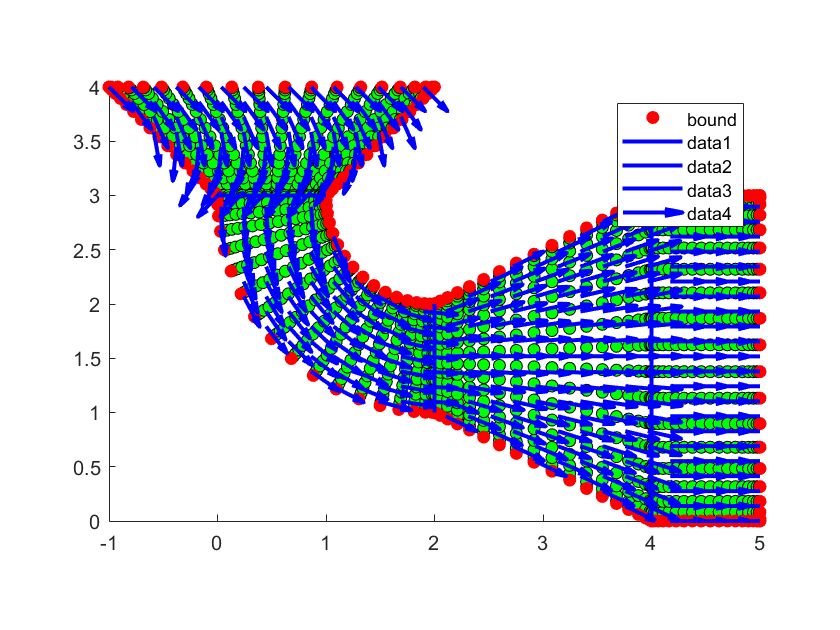
\includegraphics[scale=0.35]{F1.png}
%		\caption{Forward $\rho$ for $a = 0.01$} 
%		\label{F1}
%	\end{figure}

\begin{document}

\section*{Periodic Boundary Conditions for OCPs}
\section{Periodic Boundary Conditions 1D Advection-Diffusion}
We consider the advection diffusion equation with periodic boundary conditions and a corresponding OCP:
\begin{align*}
	&\min \frac{1}{2}|| \rho - \hr||^2 + \frac{\beta}{2}||\w||^2\\
	&\text{subject to:}\\
	&\frac{\partial \rho}{\partial t} = \frac{\partial^2 \rho}{\partial x^2} - \frac{\partial \rho \w}{\partial x}\\
	& \rho(a) = \rho(b)\\
	& \frac{\partial \rho(a)}{\partial x} - \rho(a) \w(a) = \frac{\partial \rho(b)}{\partial x}  - \rho(b) \w(b)
\end{align*}
The relevant part of the Lagrangian is then:
\begin{align*}
	\mathcal{L} &= ... -\int_0^T \int_\Omega \left(\frac{\partial \rho}{\partial t} - \frac{\partial^2 \rho}{\partial x^2} + \frac{\partial \rho \w}{\partial x}\right)q dr dt \\
	&- \int_0^T \left(-\rho(b)q_1 + \rho(a)q_1 - \frac{\partial \rho(b)}{\partial x}q_2 + \rho(b)\w(b)q_2 + \frac{\partial \rho(a)}{\partial x}q_2 - \rho(a)\w(a)q_2\right) dt.
\end{align*}
Taking partial derivatives, the relevant part of the Lagrangian is:
\begin{align*}
	\mathcal{L} = ... - \int_0^T \left[q \frac{\partial \rho}{\partial x} - \rho\frac{\partial q}{\partial x} - \rho \w q\right]_a^b -
	\left(-\rho(b)q_1 + \rho(a)q_1 - \frac{\partial \rho(b)}{\partial x}q_2 + \rho(b)\w(b)q_2 + \frac{\partial \rho(a)}{\partial x}q_2 - \rho(a)\w(a)q_2\right)dt.
\end{align*}
Taking the derivative with respect to $\rho$ gives:
\begin{align*}
	\mathcal{L}_\rho h &= ... - \int_0^T \left[q \frac{\partial h}{\partial x} - h\frac{\partial q}{\partial x} - h \w q\right]_a^b \\
	&-
	\left(-h(b)q_1 + h(a)q_1 - \frac{\partial h(b)}{\partial x}q_2 + h(b)\w(b)q_2 + \frac{\partial h(a)}{\partial x}q_2 - h(a)\w(a)q_2\right)dt
\end{align*}
Writing all terms explicitly:
\begin{align*}
	\mathcal{L}_\rho h &= ... + \int_0^T \bigg(- q(b) \frac{\partial h(b)}{\partial x} + h(b)\frac{\partial q(b)}{\partial x} + h(b) \w(b) q(b) + q(a) \frac{\partial h (a)}{\partial x} - h(a)\frac{\partial q(a)}{\partial x} - h(a) \w(a) q(a)  \\
	&h(b)q_1 - h(a)q_1 + \frac{\partial h(b)}{\partial x}q_2 - h(b)\w(b)q_2 - \frac{\partial h(a)}{\partial x}q_2 + h(a)\w(a)q_2 \bigg)dt
\end{align*}
Then considering the terms that satisfy $\frac{\partial h}{\partial x} \neq 0$ at $a$ and $b$ separately we get:
\begin{align*}
	&\int_0^T -q(b) \frac{\partial h(b)}{\partial x} + \frac{\partial h(b)}{\partial x} q_2 dt= 0\\
	& \int_0^T q(a) \frac{\partial h (a)}{\partial x} - \frac{\partial h(a)}{\partial x}q_2 dt =0
\end{align*}
	And therefore we find $q(b) = q_2$ and $q(a) = q_2$ and so: 
	\begin{align*}
		q(a) = q(b).
	\end{align*}
Then considering the terms where $h \neq 0$, again separately for $a$ and $b$ we get:
\begin{align*}
	&\int_0^T  h(b)\frac{\partial q(b)}{\partial x} + h(b) \w(b) q(b) + h(b)q_1 - h(b)\w(b)q_2 dt = 0\\
	&\int_0^T - h(a)\frac{\partial q(a)}{\partial x} - h(a) \w(a) q(a) - h(a)q_1 + h(a)\w(a)q_2 dt = 0
\end{align*}
	And using that $q(b) = q_2$ and $q(a) = q_2$ we get:
	\begin{align*}
		\frac{\partial q(b)}{\partial x} + \w(b) q(b) + q_1 - \w(b)q(b)  = 0\\
		- \frac{\partial q(a)}{\partial x} - \w(a) q(a) - q_1 + \w(a)q(a)  = 0
	\end{align*}
	and so:
	\begin{align*}
		\frac{\partial q(b)}{\partial x}  = \frac{\partial q(a)}{\partial x}. 
	\end{align*}
	Therefore, the two boundary conditions for the adjoint equation are:
	\begin{align*}
		q(a) = q(b) \quad \frac{\partial q(b)}{\partial x}  = \frac{\partial q(a)}{\partial x},
	\end{align*}
	as expected.
	
	\section{Periodic Boundary Conditions in a General Domain}
	
	We consider the advection diffusion equation with periodic boundary conditions and a corresponding OCP:
	\begin{align*}
		&\min \frac{1}{2}|| \rho - \hr||^2 + \frac{\beta}{2}||\w||^2\\
		&\text{subject to:}\\
		&\frac{\partial \rho}{\partial t} = \nabla^2 \rho - \nabla \cdot (\rho \w)\\
		& \rho|_{\partial \Omega_l} = \rho|_{\partial \Omega_r}\\
		& \rho|_{\partial \Omega_t} = \rho|_{\partial \Omega_b}\\
		&\nabla \rho \cdot \n - \rho \w \cdot \n|_{\partial \Omega_l}= \nabla \rho \cdot \n  - \rho \w \cdot \n |_{\partial \Omega_r}\\
		& \nabla \rho \cdot \n - \rho \w  \cdot \n|_{\partial \Omega_t}= \nabla \rho \cdot \n  - \rho \w \cdot \n|_{\partial \Omega_b},
	\end{align*}
	such that $\partial\Omega_l \cup \partial\Omega_r \cup \partial\Omega_t \cup \partial\Omega_b = \partial \Omega$ and the abbreviations corresponding to left, right, top and bottom respectively.
	The relevant part of the Lagrangian is then:
	\begin{align*}
		\mathcal{L} &= ... -\int_0^T \int_\Omega \left(\frac{\partial \rho}{\partial t} - \nabla^2 \rho + \nabla \cdot (\rho \w) \right)q dr dt \\
		&- \int_0^T \int_{\partial \Omega_l} \left(- \rho q_1 - \nabla \rho q_2 \cdot \n  + \rho \w q_2 \cdot \n \right) dr  + \int_{\partial \Omega_r} \left(\rho q_1 + \nabla \rho q_2 \cdot \n - \rho \w q_2\cdot \n  \right)  dr  \\
		& + \int_{\partial \Omega_t} \left(- \rho q_3 - \nabla \rho q_4 \cdot \n  + \rho \w q_4 \cdot \n  \right)  dr  + \int_{\partial \Omega_b} \left(\rho q_3 + \nabla \rho q_4 \cdot \n  - \rho \w q_4  \cdot \n \right) drdt.
	\end{align*}
	Taking partial derivatives, the relevant part of the Lagrangian is:
	\begin{align*}
		\mathcal{L} &= ... - \int_0^T \int_{\partial \Omega} \left( q \nabla \rho - \rho\nabla q - \rho \w q \right) \cdot \n  dr dt\\
		&- \int_0^T \int_{\partial \Omega_l} \left(- \rho q_1 - \nabla \rho q_2\cdot \n + \rho \w q_2\cdot \n \right)   dr  + \int_{\partial \Omega_r} \left(\rho q_1 + \nabla \rho q_2 \cdot \n- \rho \w q_2\cdot \n \right)   dr  \\
		& + \int_{\partial \Omega_t} \left(- \rho q_3 - \nabla \rho q_4 \cdot \n + \rho \w q_4 \cdot \n\right) dr  + \int_{\partial \Omega_b} \left(\rho q_3 + \nabla \rho q_4 \cdot \n - \rho \w q_4 \cdot \n \right) drdt.
	\end{align*}
	Taking the derivative with respect to $\rho$ gives:
	\begin{align*}
		\mathcal{L} &= ... - \int_0^T \int_{\partial \Omega} q \frac{\partial h}{\partial n} - h\frac{\partial q}{\partial n} - \rho \w q  \cdot \n  dr dt\\
		&- \int_0^T \int_{\partial \Omega_l} \left(- h q_1  - \frac{\partial h }{\partial n} q_2 + h \w q_2  \cdot \n \right) dr  + \int_{\partial \Omega_r} \left(h q_1 + \frac{\partial h }{\partial n}q_2 - h \w q_2 \cdot \n  \right) dr  \\
		& + \int_{\partial \Omega_t} \left(- h q_3 - \frac{\partial h }{\partial n} q_4 + h \w q_4 \cdot \n  \right) dr  + \int_{\partial \Omega_b} \left(h q_3 + \frac{\partial h}{\partial n}q_4 - h \w q_4 \cdot \n  \right) drdt.
	\end{align*}
	Writing all terms explicitly:
	\begin{align*}
		\mathcal{L} &= ... - \int_0^T \int_{\partial \Omega_l} \left( q \frac{\partial h}{\partial n} - h\frac{\partial q}{\partial n} - h \w q \cdot \n- h q_1 - \frac{\partial h }{\partial n} q_2 + h \w q_2 \cdot \n \right) dr\\
		&  + \int_{\partial \Omega_r} \left(- q \frac{\partial h}{\partial n} + h\frac{\partial q}{\partial n} + h \w q  \cdot \n + h q_1 + \frac{\partial h }{\partial n}q_2 - h \w q_2 \cdot \n \right) dr  \\
		& + \int_{\partial \Omega_t} \left(q \frac{\partial h}{\partial n} - h\frac{\partial q}{\partial n} - h \w q  \cdot \n- h q_3 - \frac{\partial h }{\partial n} q_4 + h \w q_4 \cdot \n \right) dr\\
		&  + \int_{\partial \Omega_b} \left(-q \frac{\partial h}{\partial n} + h\frac{\partial q}{\partial n} + h \w q  \cdot \n + h q_3 + \frac{\partial h}{\partial n}q_4 - h \w q_4  \cdot \n\right) drdt.
	\end{align*}
	When writing out the terms explicitly we pay attention to the fact that $n|_{\partial \Omega_l} = - n|_{\partial \Omega_r}$ and $n|_{\partial \Omega_t} = - n|_{\partial \Omega_b}$.
	Then considering the terms that satisfy $\frac{\partial h}{\partial n}$ on each boundary separately, we get:
	\begin{align*}
		&\int_0^T \int_{\partial \Omega_l} q \frac{\partial h}{\partial n}- \frac{\partial h }{\partial n} q_2 dr dt= 0 \qquad \int_0^T \int_{\partial \Omega_r} -q \frac{\partial h}{\partial n}+ \frac{\partial h }{\partial n}q_2 dr dt= 0 \\
		&\int_0^T \int_{\partial \Omega_t} q \frac{\partial h}{\partial n}- \frac{\partial h }{\partial n} q_4 dr dt= 0 \qquad \int_0^T \int_{\partial \Omega_b} -q \frac{\partial h}{\partial n}+ \frac{\partial h}{\partial n}q_4 dr dt= 0. \\
	\end{align*}
	Therefore we have 
	\begin{align*}
		&q = q_2 |_{\partial \Omega_l} \quad q =  q_2 |_{\partial \Omega_r}\\
		&q = q_4 |_{\partial \Omega_t} \quad q =  q_4 |_{\partial \Omega_b},
	\end{align*}
	and so:
	\begin{align*}
		q |_{\partial \Omega_l} = q |_{\partial \Omega_r} \quad q |_{\partial \Omega_t} = q|_{\partial \Omega_b},
	\end{align*}
	as expected.
	Now, considering $h \neq 0$ on each separate boundary gives:
	\begin{align*}
		&\int_0^T \int_{\partial \Omega_l} - h \frac{\partial q}{\partial n}  - h q \w \cdot \n - h q_1 + h q_2 \w \cdot \n dr dt = 0\\
		&\int_0^T \int_{\partial \Omega_r}  h \frac{\partial q}{\partial n}  + h q \w \cdot \n + h q_1 - h q_2 \w \cdot \n dr dt = 0 \\
		&\int_0^T \int_{\partial \Omega_t}- h \frac{\partial q}{\partial n}  - h q \w \cdot \n - h q_3 + h q_4 \w \cdot \n dr dt = 0 \\
		&\int_0^T \int_{\partial \Omega_b} h \frac{\partial q}{\partial n}  + h q \w \cdot \n + h q_3 - h q_4 \w \cdot \n dr dt = 0 .
	\end{align*}
	Using the relationships of $q$, $q_2$ and $q_4$ from above, the terms involving $\w$ cancel and we get:
	\begin{align*}
		&\int_0^T \int_{\partial \Omega_l} - h \frac{\partial q}{\partial n}   - h q_1 dr dt = 0 \qquad \int_0^T \int_{\partial \Omega_r}  h \frac{\partial q}{\partial n}  + h q_1 dr dt = 0 \\
		&\int_0^T \int_{\partial \Omega_t}- h \frac{\partial q}{\partial n}   - h q_3 dr dt = 0 \qquad
		\int_0^T \int_{\partial \Omega_b} h \frac{\partial q}{\partial n}   + h q_3  dr dt = 0 .
	\end{align*}
	This results in the four relationships:
	\begin{align*}
		\frac{\partial q}{\partial n} = - q_1 |_{\partial \Omega_l}, \quad \frac{\partial q}{\partial n} = - q_1 |_{\partial \Omega_r}, \quad
		\frac{\partial q}{\partial n} = - q_3 |_{\partial \Omega_t}, \quad
		\frac{\partial q}{\partial n} = - q_3 |_{\partial \Omega_b},
	\end{align*}
	And therefore, we get:
	\begin{align*}
		&\frac{\partial q}{\partial n}|_{\partial \Omega_l} = \frac{\partial q}{\partial n}|_{\partial \Omega_r}, \qquad \frac{\partial q}{\partial n}|_{\partial \Omega_t} = \frac{\partial q}{\partial n}|_{\partial \Omega_b},
	\end{align*}
	as required.
	
	
	%%%%%%
		
	\section{Periodic Boundary Conditions for a General Flux}
	
	We consider the advection diffusion equation with periodic boundary conditions and a corresponding OCP:
	\begin{align*}
		&\min \frac{1}{2}|| \rho - \hr||^2 + \frac{\beta}{2}||\w||^2\\
		&\text{subject to:}\\
		&\frac{\partial \rho}{\partial t} = \nabla \cdot \left(\nabla \rho - \rho \w\right) = -\nabla \cdot \jf\\
		& \rho|_{\partial \Omega_l} = \rho|_{\partial \Omega_r}\\
		& \rho|_{\partial \Omega_t} = \rho|_{\partial \Omega_b}\\
		& - \jf \cdot \n |_{\partial \Omega_l}= - \jf \cdot \n|_{\partial \Omega_r}
	\end{align*}
	such that $\partial\Omega_l \cup \partial\Omega_r = \partial \Omega$ and the abbreviations corresponding to left and right respectively. Top and bottom boundaries are omitted, since, as shown in the previous section, they follow analogously and are independent of the results on the left and right boundary. Note that we could match first derivatives instead of the flux on the boundary.
	The relevant part of the Lagrangian is then:
	\begin{align*}
		\mathcal{L} &= ... -\int_0^T \int_\Omega \left(\frac{\partial \rho}{\partial t} + \nabla \cdot \jf\right)q dr dt - \int_0^T \int_{\partial \Omega_l} \left(- \rho q_1 - \jf \cdot \n q_2 \right) dr  + \int_{\partial \Omega_r} \left(\rho q_1 +  \jf \cdot \n q_2  \right)  dr .
	\end{align*}
	Integrating by parts, and omitting terms in $\Omega$, gives:
	\begin{align*}
		\mathcal{L} &= ... - \int_0^T \int_{\partial \Omega} q \jf  \cdot \n + \mathbf{k}(\rho, q) \cdot \n  dr dt - \int_0^T \int_{\partial \Omega_l} \left(- \rho q_1 - \jf \cdot \n q_2 \right)   dr  + \int_{\partial \Omega_r} \left(\rho q_1 + \jf \cdot \n q_2 \right)   dr, 
	\end{align*}
	where $\mathbf{k}$ are any terms arising from integrating by parts a second time.
	We now need to take the Frech\'et derivative of $\jf$ with respect to $\rho$. This cannot be done in general, because $\jf$ does not only depend on $\rho$ but also on $\mathbf r$. In each case we need to calculate:
	\begin{align*}
		\jf'(h) := \jf (\rho + h) - \jf (\rho).
	\end{align*}
	Similarly, we need to take the derivative of $\mathbf k$ and denote it by $\mathbf{k}'$.
	Denoting this Frech\'et derivative by $\jf'(h)$ we can write out further terms as follows:
	\begin{align*}
		\mathcal{L}_\rho &= ... - \int_0^T \int_{\partial \Omega} q \jf'(h)   \cdot \n + \mathbf{k}' \cdot \n dr dt - \int_0^T \int_{\partial \Omega_l} \left(- h q_1 - \jf'(h)  \cdot \n q_2 \right)   dr  + \int_{\partial \Omega_r} \left(h q_1 + \jf'(h)  \cdot \n q_2 \right)   dr dt. 
	\end{align*}
	When writing out the terms explicitly we pay attention to the fact that $\n|_{\partial \Omega_l} = - \n|_{\partial \Omega_r}$ and $\n|_{\partial \Omega_t} = - \n|_{\partial \Omega_b}$.
	\begin{align*}
		\mathcal{L}_\rho &= ... - \int_0^T \int_{\partial \Omega_l} \left(- h q_1 + q \jf'(h)   \cdot \n  + \mathbf{k}' \cdot \n- \jf'(h)  \cdot \n q_2 \right)   dr  \\
		&+ \int_{\partial \Omega_r} \left(h q_1 - q \jf'(h)   \cdot \n - \mathbf{k}' \cdot \n+ \jf'(h)  \cdot \n q_2 \right)   dr dt .
	\end{align*}
	In order to proceed further, we need to split up $\jf'(h)$ into two parts as follows:
	\begin{align*}
		\jf'(h) = \jf'_1(h) + h \jf'_2,
	\end{align*}
	so that $\jf'_1$ is applied to $h$, since it depends on $\mathbf{r}$ as well (e.g. the Frech\'et derivative of $\nabla \rho$) and $\jf'_2$ is applied to another function and multiplied by $h$ (e.g. h $\frac{\partial }{\partial n}$ applied to $q$). We do the same for $\mathbf k'$.
	We then have:
	\begin{align*}
		\mathcal{L}_\rho &= ... - \int_0^T \int_{\partial \Omega_l} \left(- h q_1 + q \jf_1'(h)   \cdot \n + \mathbf{k}_1' \cdot \n - \jf_1'(h)  \cdot \n q_2  + h \jf'_2 q \cdot \n + h \mathbf{k}_2' \cdot \n-  h \jf'_2 q_2 \cdot \n \right)   dr  \\
		&+ \int_{\partial \Omega_r} \left( h q_1 - q \jf_1'(h)   \cdot \n -\mathbf{k}_1' \cdot \n+ \jf_1'(h)  \cdot \n q_2 - h\mathbf{k}_2' \cdot \n - h \jf'_2 q \cdot \n +  h \jf'_2 q_2 \cdot \n \right)   dr dt.
	\end{align*}
	Considering $\jf'_1 \neq 0$, we get:
	\begin{align*}
		\int_0^T \int_{\partial \Omega_l} \left( q \jf_1'(h)   \cdot \n  + \mathbf{k}_1' \cdot \n - \jf_1'(h)  \cdot \n q_2  \right)   dr  + \int_{\partial \Omega_r} \left(-q \jf_1'(h)   \cdot \n - \mathbf{k}_1' \cdot \n + \jf_1'(h)  \cdot \n q_2  \right)   dr dt = 0 .
	\end{align*}
	Note that if $\mathbf{k}_1' = 0$, we can conclude that $q = q_2$ on both boundaries.
	In general, $q_2|_{\partial \Omega_l} = q_2|_{\partial \Omega_r}$, i.e. $q_2$ is constant on the boundary, and an equivalent statement holds for $q_1$. Therefore, we have that:
	\begin{align*}
		\int_0^T \int_{\partial \Omega_l}  q \jf_1'(h)   \cdot \n  +\mathbf{k}_1' \cdot \n   dr dt = \int_0^T \int_{\partial \Omega_r} q \jf_1'(h)   \cdot \n  +  \mathbf{k}_1' \cdot \n  dr dt .
	\end{align*}
	Writing this in terms of the integrand only can be done for each specific case of $\jf_1'$ and $\mathbf{k}_1'$. 
	Now considering all terms such that $h \neq 0$ on each boundary separately, we get:
	\begin{align*}
		&\int_0^T \int_{\partial \Omega_l} \left(- h q_1  + h \jf'_2 q \cdot \n + h\mathbf{k}_2' \cdot \n-  h \jf'_2 q_2 \cdot \n \right)   dr  dt =0 \\
		&\int_0^T \int_{\partial \Omega_r} \left( h q_1  - h \jf'_2 q \cdot \n - h\mathbf{k}_2' \cdot \n + h \jf'_2 q_2 \cdot \n \right)   dr  dt =0 ,
	\end{align*}
	and so, as in the previous sections, we have:
	\begin{align*}
		q_1 &=   \jf'_2 q \cdot \n + \mathbf{k}_2' \cdot \n - \jf'_2 q_2 \cdot \n |_{\partial \Omega_l} \\
		q_1 &=  \jf'_2 q \cdot \n + \mathbf{k}_2' \cdot \n -\jf'_2 q_2 \cdot \n |_{\partial \Omega_r}, 
	\end{align*}
	which gives:
	\begin{align*}
		\jf'_2 q \cdot \n +  \mathbf{k}_2' \cdot \n - \jf'_2 q_2 \cdot \n |_{\partial \Omega_l} =  \jf'_2 q \cdot \n + \mathbf{k}_2' \cdot \n - \jf'_2 q_2 \cdot \n |_{\partial \Omega_r}.
	\end{align*}
	If $\mathbf{k}_1' = 0$ and so $q = q_2$ as discussed above, the two terms involving $\jf_2'$ cancel and we get
	\begin{align*}
		\mathbf{k}_2' \cdot \n  |_{\partial \Omega_l} =   \mathbf{k}_2' \cdot \n  |_{\partial \Omega_r}.
	\end{align*}
	Otherwise, since $q_2|_{\partial \Omega_l} = q_2|_{\partial \Omega_r}$, we can at least conclude that:
	\begin{align*}
		\jf'_2 q \cdot \n + \mathbf{k}_2' \cdot \n  |_{\partial \Omega_l} =  \jf'_2 q \cdot \n + \mathbf{k}_2' \cdot \n  |_{\partial \Omega_r}.
	\end{align*}
	\\
	\\
	An example: Let $\jf = \nabla \rho - \rho \w$ as above. Then we have that $\jf_1'(h) = \nabla h$ and $\jf_2' = \w $. From integration by parts we will get that $\mathbf k = - \rho \nabla q$, so $\mathbf k_1' = 0$ and $\mathbf k_2' = -  \nabla q$.
	We therefore get that:
	\begin{align*}
		& \nabla q \cdot \n |_{\partial \Omega_l} = \nabla q \cdot \n |_{\partial \Omega_r},
	\end{align*}
	and
	\begin{align*}
		\int_0^T \int_{\partial \Omega_l}  q \nabla h   \cdot \n    dr dt = \int_0^T \int_{\partial \Omega_r} q \nabla h  \cdot \n    dr dt,
	\end{align*}
	and so 
	\begin{align*}
		q |_{\partial \Omega_l} = q|_{\partial \Omega_r},
	\end{align*}
	as required.
\end{document}